% !TEX root = ../../Tesi_Triennale_PMNS.tex
\chapter[cWB]{cWB: proprietà dell'algoritmo per la rivelazione e la ricostruzione di segnali di onde gravitazionali}
\label{chapter:cwb}

I metodi coerenti le statistiche vengono calcolate come somma coerente delle risposte dei detector singoli. Gli algoritmi che sfruttano questi metodi devono risultare più efficienti, devono cioè avere una probabilità di falso allarme più bassa, rispetto alle statistiche calcolate sulle risposte di ogni detector singolarmente.

L'algoritmo che si utilizza, Coherent WaveBurst (cWB), differisce dai metodi tradizionali che identificano gli eventi nei detector singolarmente usando statistiche di eccesso di potenza e poi verificano la coerenza tra i segnali nei vari detector. Esso utilizza infatti i dati di tutti i detector in un'unica statistica coerente costituita da una analisi della massima likelihood. 
I vantaggi di questo tipo di analisi sono molteplici: innanzitutto la sensibilità del metodo non sarà limitata dal detector meno sensibile nel network, in quanto la likelihood utilizzata nei metodi coerenti rappresenta il rapporto segnale su rumore (SNR) totale del segnale ricostruito/rivelato dal network. Inoltre questo metodo permette di costruire altre statistiche coerenti, come il null stream o il coefficiente di correlazione  del network, per distinguere segnali che effettivamente hanno una controparte fisica rispetto a eccessi di rumore ambientale o strumentale. Infine è possibile ricostruire la posizione celeste della sorgente.
\section{Analisi coerente}
\label{section:coherent_analysis}
La pipeline di cWB per rivelare e ricostruire segnali utilizza un metodo basato sul funzionale rapporto di verosimiglianza, che, in un'ipotesi idealistica di rumore gaussiano quasi stazionario, può essere scritto nel dominio di wavelet (in un piano tempo-frequenza) come
\begin{equation}
	\mathcal{L} = \sum_{k=1}^{K}\sum_{i,j=1}^{N}\left(\frac{w_k^2[i,j]}{\sigma_k^2[i,j]} - \frac{(w_k[i,j]-\xi_k[i,j])^2}{\sigma_k^2[i,j]}  \right)
	\label{eqn:Likelihood}
\end{equation}
dove K è il numero di detector nel network, $w_k[i,j]$ è il campione di dati del detector (l'indice i itera sui tempi, mentre l'indice j itera sulle frequenze) e infine $\xi_k[i,j]$ è la risposta del detector k-esimo.
Il rumore del detector è è caratterizzato dalla deviazione standard $\sigma_k[i,j]$ che può variare lungo il piano tempo-frequenza.
Le risposte del network sono scritte come
\begin{equation}
	\xi_k[i,j] = F_{+,k}h_+[i,j] + F_{\times,k}h_\times[i,j]
	\label{eqn:detector_response}
\end{equation}
dove $h_{+}[i,j]$ e $h_{\times}[i,j]$ sono le ampiezze delle due polarizzazioni della GW e $F_{+,k}(\theta,\phi)$ e $F_{\times,k}(\theta,\phi)$ sono gli antenna pattern del detector k-esimo\cite{Klimenko_2008}. Gli antenna pattern descrivono come il detector riceve l'energia in funzione della posizione angolare. *Breve descrizione antenna pattern* *immagine antenna pattern di uno dei rivelatori*\cite{Schutz_2011}.

Dunque, al variare di $h_{+}[i,j]$ e $h_{\times}[i,j]$ varia anche $\mathcal{L}$, l'obiettivo è quindi ottenere i valori delle ampiezze che massimizzano il funzionale di verosimiglianza e quindi si deduce la forma d'onda nel dominio dei tempi facendo una trasformazione di wavelet inversa.%, che consisterà dunque 

Per semplicità si introducono i seguenti vettori:
\[
	\textbf{w}[i,j] = \left(\frac{w_1[i,j]}{\sigma_1[i,j]},\dots, \frac{w_K[i,j]}{\sigma_K[i,j]} \right) ;
	\quad
	\textbf{f}_{+(\times)}[i,j] = \left(\frac{F_{1+(\times)}[i,j]}{\sigma_1[i,j]},\dots, \frac{F_{K+(\times)}[i,j]}{\sigma_K[i,j]} \right) 
\]
mentre con la notazione $\sum_{\Omega_{TF}} = \sum_{i,j=1}^N$, in quanto si scriverà $\Omega_{TF}$ come il dominio tempo-frequenza. 

Il funzionale rapporto di verosimiglianza in equazione \ref{eqn:Likelihood} si può scrivere come
\begin{equation}
	\mathcal{L} = \mathcal{L}_+ + \mathcal{L}_\times = \sum_{\Omega_{TF}}\left[ \textbf{w} \cdot \textbf{f}_+ - \frac{1}{2}|\textbf{f}_+|^2h_+^2\right] + \sum_{\Omega_{TF}}\left[ \textbf{w} \cdot \textbf{f}_\times - \frac{1}{2}|\textbf{f}_\times|^2h_\times^2\right]
	\label{eqn:label_separated}
\end{equation}
dove i vettori di antenna pattern $\textbf{f}_+$ e $\textbf{f}_\times$ sono definiti nel Dominant Polarisation wave Frame (DPF), ovvero il piano in cui entrambi gli antenna pattern sono reali e definiti positivi e vale $\textbf{f}_+ \cdot \textbf{f}_\times = 0$. Alla luce di questo per ottenere la massima likelihood si dovrà risolvere le equazioni:
%\begin{equation}
%	\begin{cases}
%		\textbf{w} \cdot \textbf{f}_+ = |\textbf{f}_+|^2h_+ \\
%		\textbf{w} \cdot \textbf{f}_\times = |\textbf{f}_+|^2h_\times 
%	\end{cases}
%\end{equation}
\begin{equation}
	\textbf{w} \cdot \textbf{f}_+ = |\textbf{f}_+|^2h_+ \quad\quad\quad  \textbf{w} \cdot \textbf{f}_\times = |\textbf{f}_+|^2h_\times 
	\label{eqn:sistema_soluzione}
\end{equation}

\paragraph{Regolatori} C'è una particolare classe di vincoli, i regolatori, che dipendono da come il network reagisce a un determinato segnale.

\subsection{Trasformazioni di wavelet}
\label{subsection:wavelet_transform}
\begin{wrapfigure}{r}{0.45\textwidth}
	\vspace{-15pt}
	\begin{center}
		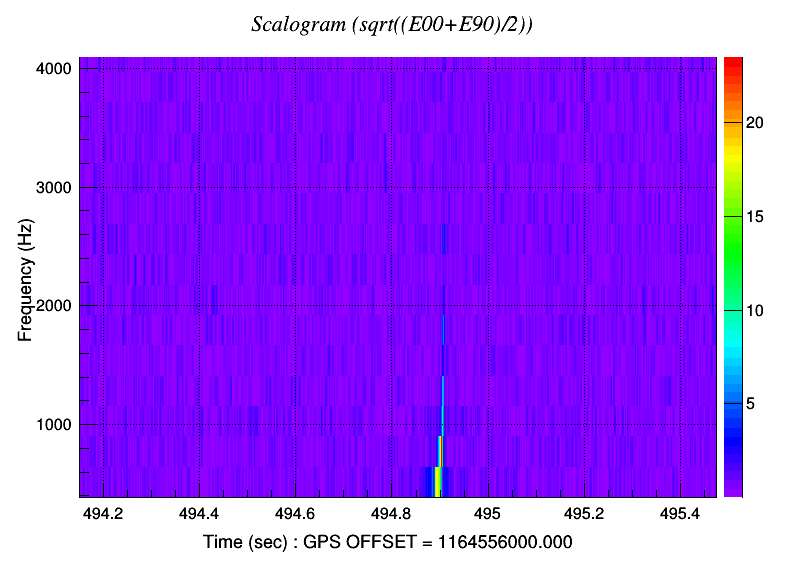
\includegraphics[width=0.5\textwidth]{figures/Capitolo_3/L1_scalogram_0.png}
	\end{center}
	\vspace{-5pt}
	\caption{Scallogramma ottenuto da una analisi di una simulazione di coalescenza di una BNS con EOS SHT2.0 con rumore gaussiano del detector LIGO Hanford}
	\label{fig:scalogram_example}
	\vspace{-40pt}
\end{wrapfigure}
Le trasformazioni di wavelet, partendo dai dati discreti, producono serie di dati $w[i,j]$ nel piano tempo-frequenza. Lo spettro di wavelet può essere quindi rappresentato con uno scallogramma tempo-frequenza. La risoluzione nel dominio del tempo $\Delta t_j(R)$ è determinata dal rate di campionamento R e dall'indice di scala j. Poiché le trasformazioni di wavelet costituiscono una serie di trasformazioni di Fourier infinitesime, conservano il volume del campione, pari a 1/2 per la serie temporale in input. Si avrà quindi una risoluzione in frequenza $\Delta f_j$ definita come 1/(2$\Delta t_j$) che determina la larghezza di banda per l'indice j. Per ottimizzare la ricerca nel piano, cWB procede con diverse trasformazioni a risoluzioni diverse, che permette di ottenere il grafico in figura \ref{fig:scalogram_example}.
\subsection{Filtro di predizione lineare dell'errore}



%Introduzione sull'algoritmo fatta nel paragrafo precedente, magari riprenderla veltocemente.

%Coherent analysis, significato e descrizione della likelihood: spiega quindi bene la differenza con gli algoritmi classici di confronto con segnali già modellati.

%regolatori, antenna pattern

%algoritmi utilizzati: wavelet transformation, (linear predicion error), mappa verosimiglianza, mappa energia coerente (con piccoli grafici esemplificativi)

%(cenni sulla trasformazione di fase)

\begin{center}
	\begin{figure}[ht]
		\centering
		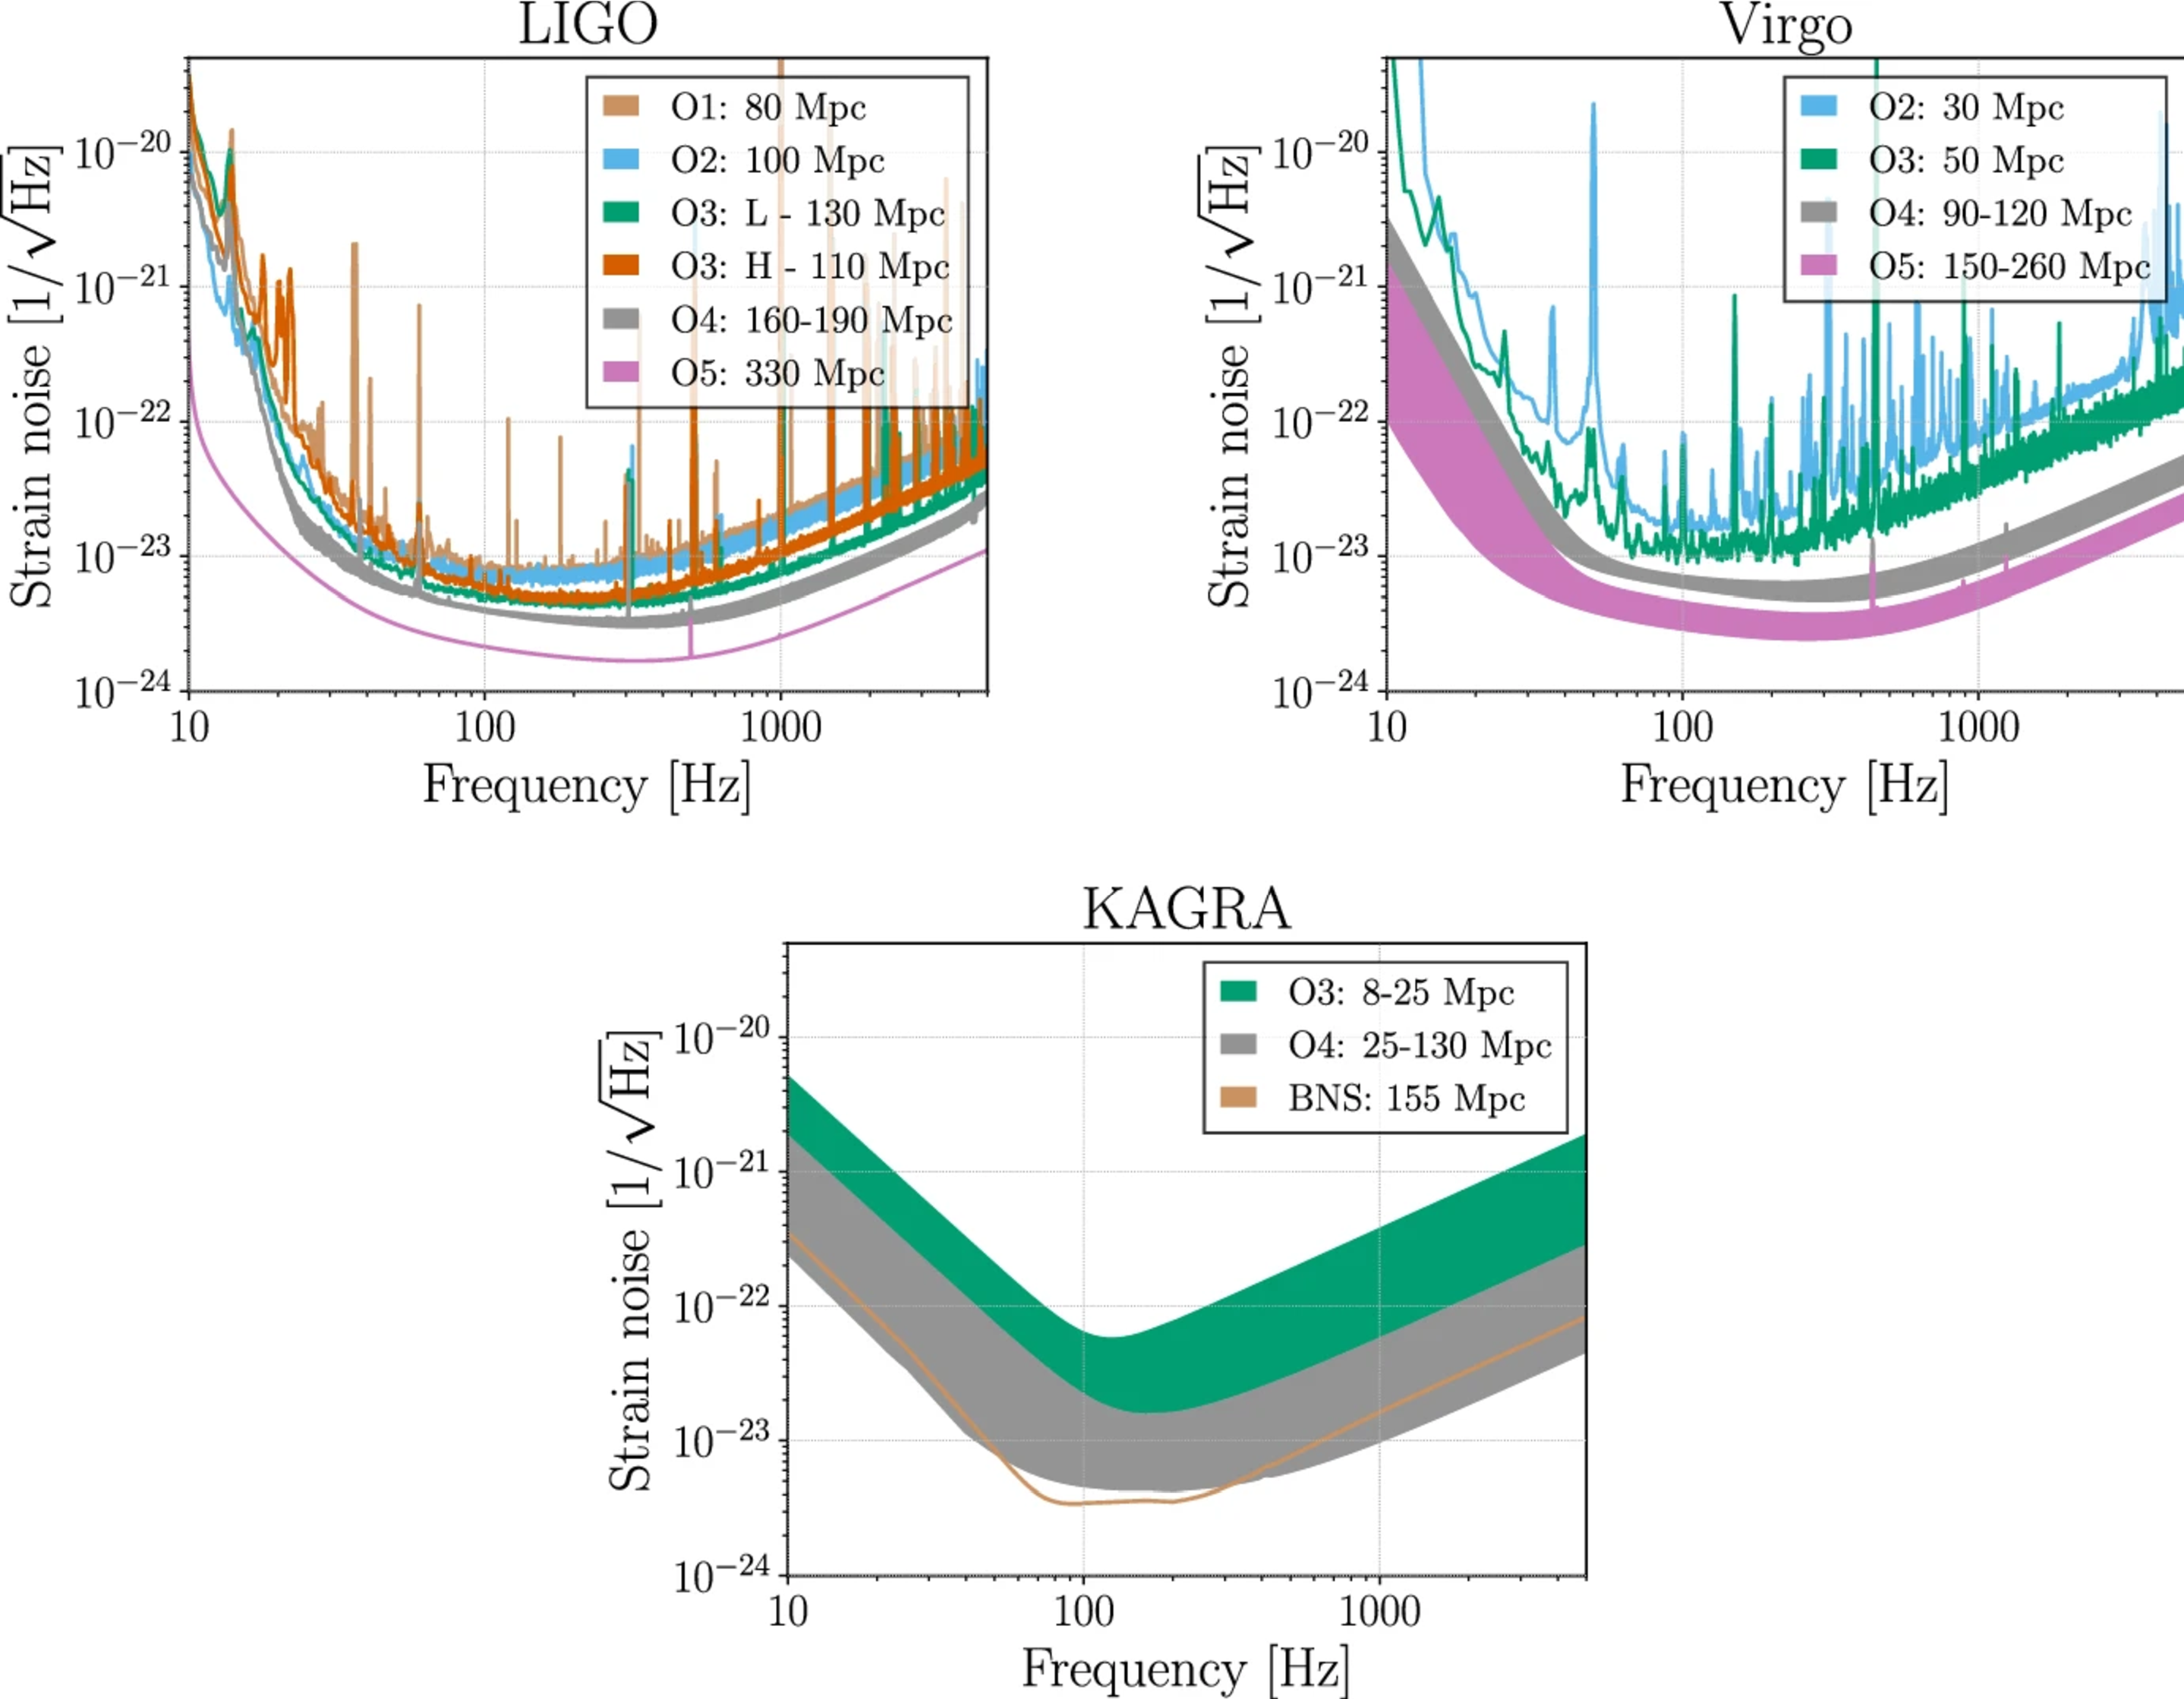
\includegraphics[scale=0.25, angle=0]{figures/Capitolo_3/noiseO4.pdf}
		\setlength{\belowcaptionskip}{-20pt}
		\caption{Prospetti \cite{Abbott_2020a}}
		\label{fig:noiseO4}
	\end{figure}
\end{center}

\lipsum[3]\cite{Abbott_2017a}.

\lipsum[4]\cite{Klimenko_2008}.

\lipsum[6]\cite{Klimenko_2016}.